%       INTRO
%       TRANSFORMÉE MULTI-ÉCHELLE
%       HEURISTIQUES D'ADAPTATION
%       ALGORITHMES
%           CALCULS NIVEAU COURANT
%           CALCUL NIVEAU FIN
%       SOURCES D'ERREURS
%       IMPLÉMENTATIONS
%           MÉTHODES CLASSIQUES 
%           SAMURAI

La multi-résolution adaptative (MRA) est une méthode très efficace pour les problèmes multi-échelles. 
L'objectif est de concentrer les efforts computationnels là où ils sont nécessaires. 
Concrètement cela consiste à augmenter la résolution de la grille de calcul où la solution est complexe et la diminuer où la solution est simple à décrire.
La MRA est donc une méthode de HPC (\textit{high performance computing}) puisqu'elle vise à optimiser l'allocation des ressources de calcul.\par
Cette partie introduit le lecteur à cette méthode en présentant d'abord le concept mathématique de transformée multi-échelle (ou transformée en ondelette)
qui est à la base de la MRA. 
Puis il est expliqué comment la transformée multi-échelle permet d'adapter le maillage pour optimiser la charge computationnelle.
Une fois ces prérequis établis, l'algorithme typique de mise en oeuvre de la multi-résolution adaptative est décrit.
S’ensuit alors naturellement une présentation des différentes implémentations de la MRA, avec une attention particulière sur celle développée au CMAP au travers 
du logiciel Samurai.
Enfin l'impact de la multi-résolution sur la qualité des solutions numériques est abordé. 

\subsubsection{La transformée multi-échelle}
    Cette partie présente la transformée multi-échelle discrète. La transformée multi-échelle continue en simulation numérique,
    c'est bien sûr la version discrète qui est utile.
    Elle se veut avant tout introductive et omets ou simplifie certaines notions; plus de détails sont donnés en \cite{postePoly}.

    \paragraph{Définition mathématique}
        Les explications sont développées en dimensions un à des fins pédagogiques, la plupart des concepts s'entendent naturellement aux dimensions supérieures. 
        De plus, la discrétisation de l'espace se fait selon une grille dyadique, d'autre choix pourraient être fait mais c'est un choix simple, naturel et standard.
        Il faut détailler cette notion.
        \begin{definition}[Grille dyadique]
            Une grille dyadique ou discrétisation dyadique d'un intervalle $I \subset \mathbb R$ est une série de partitions de $I$ indexées 
            par des entiers $j \in J \subset \mathbb N^*$.
            La discrétisation de niveau $j$ correspond à une partitions de $I$ en $2^j$ intervalles (voir fig. \ref{fig:schema_sdyadique}). Ainsi à chaque changement de niveau, du niveau $j$ vers le niveau $j+1$,
            la résolution de la discrétisation est doublée. Les cases de cette partition dyadique sont indexées par deux entiers: $j$ le niveau de résolution de la grille
            et $k$ l'index de la case au sein de ce niveau. En particulier les cases $2k$ et $2k+1$ du niveau $j+1$ correspondent à la case $k$ du niveau $j$.
        \end{definition}
        \begin{figure}[htbp]
    \centering
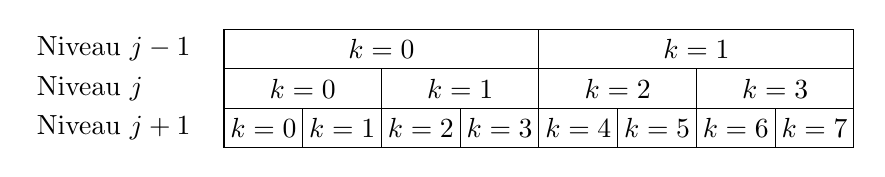
\begin{tikzpicture}


\node[anchor=west] at (-6.5, -.25) {Niveau $j+1$};
\node[anchor=west] at (-6.5, .25) {Niveau $j$};
\node[anchor=west] at (-6.5, .75) {Niveau $j-1$};
% Niveau j-1

\draw (-4,.5) rectangle (0,1);
\draw (0,.5) rectangle (4,1);

    % Niveau j
\draw (-4,0) rectangle (-2,.5);
\draw (-2,0) rectangle (0,.5);
\draw (0,0) rectangle (2,.5);
\draw (2,0) rectangle (4,.5);
%\node at (1,1.75) {$k=2$};

% Niveau j+1

\draw (-4,-.5) rectangle (-3,0);
\draw (-3,-.5) rectangle (-2,0);
\draw (-2,-.5) rectangle (-1,0);
\draw (-1,-.5) rectangle (0,0);
\draw (0,-.5) rectangle (1,0);
\draw (1,-.5) rectangle (2,0);
\draw (2,-.5) rectangle (3,0);
\draw (3,-.5) rectangle (4,0);

% Relations
\node at (-2, .75) {$k=0$};
\node at (+2, .75) {$k=1$};

\node at (-3, .25) {$k=0$};
\node at (-1, .25) {$k=1$};
\node at (+1, .25) {$k=2$};
\node at (+3, .25) {$k=3$};

\node at (-3.5, -.25) {$k=0$};
\node at (-2.5, -.25) {$k=1$};
\node at (-1.5, -.25) {$k=2$};
\node at (-0.5, -.25) {$k=3$};

\node at (+0.5, -.25) {$k=4$};
\node at (+1.5, -.25) {$k=5$};
\node at (+2.5, -.25) {$k=6$};
\node at (+3.5, -.25) {$k=7$};


\end{tikzpicture}
\caption{Exemple de grille dyadique}
\label{fig:schema_sdyadique}
\end{figure}
        Dans ce qui suit il est supposé sans perte de généralité que la discrétisation se fait sur l'intervalle $[0,1]$,
        ainsi le niveau $j$ correspond à des cellules de tailles $1/{2^j}$ et la cellule $k$ du niveau $j$ est centrée en
        $x_k^j = \frac{k+(k+1)}{2} \frac{1}{2^j} = \frac{2k+1}{2^j}.$
        La notion d'ondelette se définit de la manière suivante:
        \begin{definition}[Ondelette]
            Une ondelette est une fonction $\Phi \in L^2(\mathbb R)$ à support compact de moyenne nulle.
            Pour qu'une ondelette soit pertinente dans le cas de la transformée en multi-échelle il est requis
            que la famille $\Bigl(x \mapsto \Phi( 2^j k - x ) \bigr)_{ (j,k)\in \mathbb{Z} \times \mathbb{Z} }$ forme une base de $L^2(\mathbb{R})$.
            En effet la transformée en ondelette sera une projection sur cette base, un peu comme la transformée de Fourrier est une projection sur les 
            fonctions trigonométriques.
        \end{definition}
        Alors la transformée en ondelette discrète peut être définie:
        \begin{definition}[Transformée en ondelette discrète - \textit{Discrete Wavelet Transform, DWT}] Donnée une fonction $f$,
            le coefficient $\gamma_k^j$ de sa DWT sur la cellule $k$ au niveau de résolution $j$ est:
            \begin{align}
                &\gamma_k^j = \frac{1}{N_j} \int_\mathbb{R} \Phi(2^j\cdot k - t)f(t) \text{d} t,\\\notag
                &\text{Où $N_j$ est un coefficient normalisation dépendant du niveau $j$.}
            \end{align}
            Contrairement à une transformée de Fourier, les coefficients ne dépendent pas d'une mais de deux variables. En effet, 
            la transformée en ondelette est plus riche d'informations. Là où la transformée de Fourier ne donne qu'une information 
            sur le contenu fréquentiel d'un signal, la transformée en ondelette donne une information sur le contenu en fréquence \underline{et}
            sur la localisation de ce contenu fréquentiel.
            L'indice $j$ de \textit{dilatation} fixe l'échelle analysée, c'est à dire la longueur d'onde analysée. Par exemple si $j=5$, 
            les coefficients $\gamma^5_k$ donne une information sur l'information portée par les longueurs d'onde de l'ordre de $2^{-5} = 1/32$.
            La variable $k$ précise l'indice de la cellule analysée.
            Par exemple $\Vert \gamma^5_10 \Vert > \Vert \gamma^5_5 \Vert$ signifie que l'information portée par l'échelle $1/32$
            est plus importante au voisinage de la case $10$ qu'au voisinage de la case $5$.
            De même si $\Vert \gamma^j_7 \Vert > \Vert \gamma^{j+1}_{14} \Vert$ cela signifie qu'au voisinage de $x=\frac{7}{2^j}$
            les longueurs d'ondes $\frac{1}{2^j}$ sont plus présentes que les longueurs d'ondes $\frac{1}{2^{j+1}}.$
            Pour se fixer les idées, c'est comme si la transformée de Fourrier n'avait qu'une vision globale du contenu en fréquence, 
            quelle ne voyait que la moyenne sur le domaine de la transformée en ondelette pour chaque longueur d'onde.
            \begin{align}
                \Vert TF\bigl[ f \bigr](\omega = 2^j) \Vert^2 \sim \Vert \sum_{k} \gamma^j_k \Vert^2.
            \end{align}
        \end{definition}

    \paragraph{}
\subsubsection{L'adaptation}
    \paragraph{}
    \paragraph{}
\subsubsection{Algorithmes de simunlation numérique}
    \paragraph{}
    \paragraph{}
\subsubsection{Impact sur les solutions}
    \paragraph{}
    \paragraph{}
\subsubsection{Implémentations de la multi-résolution}
    \paragraph{Méthodes usuelles}
    \paragraph{Le logiciel Samurai}